\documentclass{article}
 
\usepackage[spanish]{babel}
\usepackage{listings}
\usepackage{epsfig} 
\usepackage{float}
 \usepackage{hyperref}
 \usepackage{color}

%\usepackage{multicol}
%\usepackage{url}
%\renewcommand{\UrlFont}{\small}
\setlength{\parskip}{1cm}
\setlength{\parindent}{0pt}


\title{Tipos De Grafos}
\author{Héctor Hugo García López}
%\institute{PISIS UANL}
%\email{hhector.garcialpz@uanl.edu.mx}
\date{}


\begin{document}
\maketitle

\section*{Introducción}
Un grafo esta formado por un conjunto de nodos que llamaremos $N$, y un conjunto de la forma $(u,v)$ llamado aristas al que nos referiremos por $A$. Dada su composición es conveniente ver un grafo como un dibujo. Los grafos se pueden usar para ilustrar procesos, rutas, cambios de estados en ciertos procesos  y hasta un árbol genealógico. En este documento se mostrará los tipos grafos, cuales son las condiciones que tienen que cumplir y un ejemplo de su aplicación.

Para hacer una mejor referencia a los grafos, los vamos a dibujar en python y para eso necesitamos hacer uso de dos librerias, como se presenta a continuación.

\definecolor{mygreen}{rgb}{0,0.6,0}
\definecolor{mygray}{rgb}{0.5,0.5,0.5}
\definecolor{mymauve}{rgb}{0.58,0,0.82}
\lstset{ 
  backgroundcolor=\color{white},   % choose the background color; you must add \usepackage{color} or \usepackage{xcolor}; should come as last argument
  basicstyle=\footnotesize,        % the size of the fonts that are used for the code
  breakatwhitespace=false,         % sets if automatic breaks should only happen at whitespace
  breaklines=true,                 % sets automatic line breaking
  captionpos=b,                    % sets the caption-position to bottom
  commentstyle=\color{mygreen},    % comment style
  deletekeywords={...},            % if you want to delete keywords from the given language
  escapeinside={\%*}{*)},          % if you want to add LaTeX within your code
  extendedchars=true,              % lets you use non-ASCII characters; for 8-bits encodings only, does not work with UTF-8
  firstnumber=1,                % start line enumeration with line 1000
  frame=single,	                   % adds a frame around the code
  keepspaces=true,                 % keeps spaces in text, useful for keeping indentation of code (possibly needs columns=flexible)
  keywordstyle=\color{blue},       % keyword style
  language=Octave,                 % the language of the code
  morekeywords={*,...},            % if you want to add more keywords to the set
  numbers=left,                    % where to put the line-numbers; possible values are (none, left, right)
  numbersep=5pt,                   % how far the line-numbers are from the code
  numberstyle=\tiny\color{mygray}, % the style that is used for the line-numbers
  rulecolor=\color{black},         % if not set, the frame-color may be changed on line-breaks within not-black text (e.g. comments (green here))
  showspaces=false,                % show spaces everywhere adding particular underscores; it overrides 'showstringspaces'
  showstringspaces=false,          % underline spaces within strings only
  showtabs=false,                  % show tabs within strings adding particular underscores
  stepnumber=1,                    % the step between two line-numbers. If it's 1, each line will be numbered
  stringstyle=\color{mymauve},     % string literal style
  tabsize=2,	                   % sets default tabsize to 2 spaces
  title=\lstname                   % show the filename of files included with \lstinputlisting; also try caption instead of title
}

\lstinputlisting[language=Python, firstline=1, lastline=2]{PrimerProyecto.py}

%UNO...............
\section{Grafo simple no dirigido acíclico}
Primeramente se definirá ciertos conceptos. Un camino es un subconjunto de $A$ (que puede ser $A$) y recorre un subconjunto de $N$ (que puede incluir todo $N$). Un ciclo es un camino que une por lo menos 3 nodos distintos, y el nodo de inicio es el mismo que el nodo final.

En la figura \ref{1} se representa un isómero de carbono, en el cual los nodos son los diferentes elementos del compuesto, y las aristas son los enlaces que tienen un elemento con otro.

\begin{figure}[H]
\centering
\includegraphics [width=100mm] {Primero.eps}
\caption{Grafo no dirigido acíclico}
\label{1}
\end{figure}

El código que da paso a la figura antes mencionada es el siguiente.
\lstinputlisting[language=Python, firstline=11, lastline=19]{PrimerProyecto.py}
La última linea del código se usa para guardar una imagen tipo extensión eps.

%DOS........"O"
\section{Grafo simple no dirigido cíclico}
En la sección anterior se vió que es un ciclo en un grafo, en la figura \ref{2} se observa un grafo que representa la caja de cambios de un carro, donde el nodo \"O\" es estar en neutral. 

Es no dirigido porque es lo mismo si pasa de la primera marcha a la segunda, análogamente con las demás marchas; es cíclica ya que eso se repite muchas veces durante un mismo trayecto.

\begin{figure}[H]
\centering
\includegraphics [width=90mm] {Segundo.eps}
\caption{Grafo no dirigido cíclico}
\label{2}
\end{figure}
 
%Para graficar esta red, se hizo como un grafo completo dado un cambio de marcha puede ir con cualquier otro cambio excepto reversa. El código es el siguiente.

%\lstinputlisting[language=Python, firstline=22, lastline=28]{PrimerProyecto.py}

%TRES...........Preguntar parentesis
\section{Grafo simple no dirigido reflexivo}
Un nodo reflexivo es el que tiene un arista que va hacia sí mismo, es decir, para cualquier $u \in V$ existe $(u,u) \in A$. Entonces se puede decir que un grafo reflexivo es el que tiene nodos reflexivos. 
En este documento los nodos reflexivos son de color rojo.

En el siguiente ejemplo \ref{3} se tiene el horario de cierto profesor, los nodos muestran las materias y las aristas las horas que da de clase en una semana especifica. Se puede apreciar que las materias de Calculo 1, Algebra y 
Conjuntos hay repeticiones (porque están de color rojo) lo que quiere decir que después de ir, por ejemplo, a Algebra, la siguiente clase podría ser Algebra, o salir de esa clase e ir a otra distinta.

\begin{figure}[H]
\centering
\includegraphics [width=90mm] {Tercero.eps}
\caption{Grafo no dirigido reflexivo}
\label{3}
\end{figure}

Para llevar a cabo este grafo se hizo dos conjuntos llamados nodos1 y nodos2, en las siguientes lineas (15) y (17) al dibujar nodos1 y nodos2 se le asignan los colores y las posiciones ya establecidas en 
el diccionario pos
\lstinputlisting[language=Python, firstline=31, lastline=55]{PrimerProyecto.py}

%CUATRO..............
\section{Grafo simple dirigido acíclico}
Un grafo dirigido es aquel que se especifica la dirección de la arista, es decir, si $(u,v) \in A$ entonces  $(v,u) \notin A$.

Un ejemplo para la figura \ref{4} puede ser un centro de distribución de materiales, que entrega a varios proveedores que simbolizan los nodos y cada arista es el flujo de material. 

Para que este ejemplo sea considerado como un grafo simple solo se puede enviar material.
 
\begin{figure}[H]
\centering
\includegraphics [width=90mm] {Cuarto.eps}
\caption{Grafo dirigido acíclico}
\label{4}
\end{figure}

Para realizar el grafo se hizo uso de la función DiGraph() y con ella las aristas se vuelven dirigidas
\lstinputlisting[language=Python, firstline=58, lastline=64]{PrimerProyecto.py}

%CINCO..........
\section{Grafo simple dirigido cíclico}
Al igual que en el grafo no dirigido, este grafo tiene la característica de que contiene un ciclo. Si queremos representar como diagrama de flujo, un videojuego que se elige entrar 
solo (solitario) o en grupo (cooperativo) y después de esa opción se va a jugar, y cuando termina el juego, se devuelve al menú principal. 

En la figura \ref{5} se aprecia el ciclo y las flechas que nos dice que es un grafo dirigido

\begin{figure}[H]
\centering
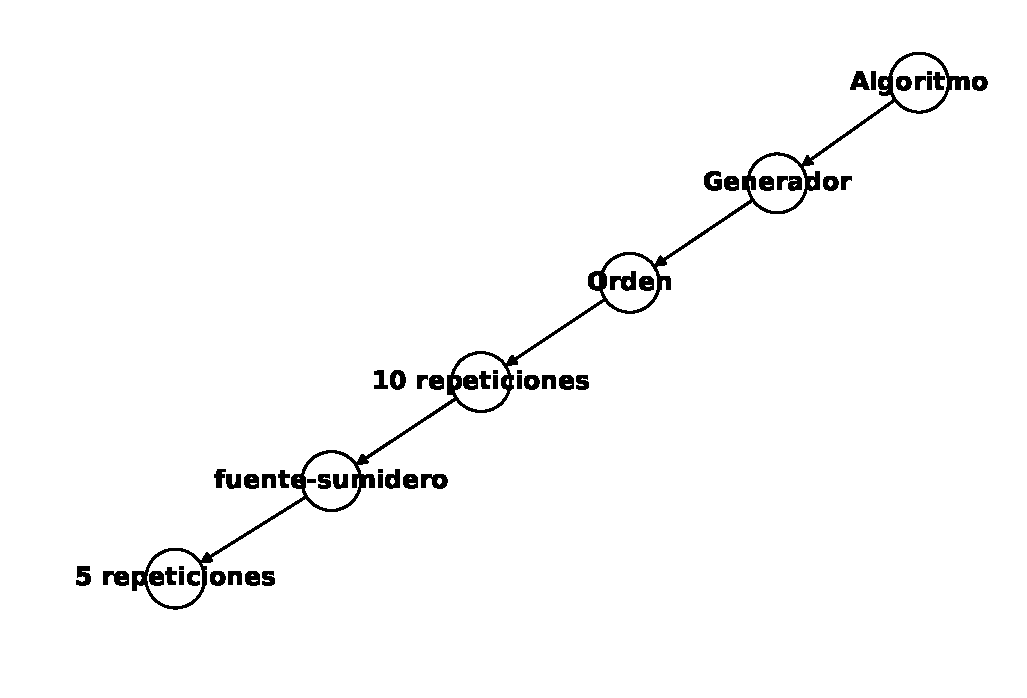
\includegraphics [width=100mm] {Quinto.eps}
\caption{Grafo dirigido cíclico}
\label{5}
\end{figure}

%\lstinputlisting[language=Python, firstline=67, lastline=75]{PrimerProyecto.py}


%SEIS............Pendiente
\section{Grafo simple dirigido reflexivo}
Supongamos que se tiene el diagrama de flujo de los procesos para la elaboración de productos en una empresa. El primer paso es la recepción donde se verifica la calidad de los productos
que entran y se cuentan los mismos con el fin de ver si lo que llegó es lo que se pidió. En caso de no cumplir con el conteo, se vuelve a verificar. Si está en mal estado se puede llevar a calidad 
e intentar recuperar el producto, pero si el producto no queda del todo bien, sigue entrando a calidad.

Este caso puede ser representado mediante un grafo, como lo muestra la figura \ref{6} donde los nodos representan los procesos y las aristas es el flujo de los productos. Los nodos reflexivos 
son como el nodo 1 o calidad, que pueden entrar varias veces al mismo proceso.

\begin{figure}[H]
\centering
\includegraphics [width=80mm] {Sexto.eps}
\caption{Grafo dirigido reflexivo}
\label{6}
\end{figure}

%SIETE...........
\section{Multigrafo no dirigido acíclico}
Un multigrafo es un grafo en el cual puede haber mas de un arista entre cada par de nodos, esto es, tiene multiplicidades en sus nodos. Gráficamente se representa con dos lineas, pero en los 
siguientes gráficos solo se muestra una linea.

Este tipo de grafos se pueden usar para representar los vuelos de cierto tipo de aerolínea entre algunos países, como lo representa en la figura \ref{7} donde los nodos son los países
y las aristas son la cantidad de vuelos.

\begin{figure}[H]
\centering
\includegraphics [width=90mm] {Septimo.eps}
\caption{Multigrafo no dirigido acíclico}
\label{7}
\end{figure}

Para dibujar estos grafos se usa la función de networkx MultiGraph() que te permite agrgar aristas que, aunque vistos como conjuntos son iguales, importan porque representan flujos (cantidades de vuelos
en nuestro ejemplo) diferentes
\lstinputlisting[language=Python, firstline=95, lastline=104]{PrimerProyecto.py}

%OCHO............
\section{Multigrafo no dirigido cíclico}
Al igual que en el grafo simple, este grafo contiene por lo menos un ciclo. Para visualizarlo mejor se hace referencia al ejemplo anterior, en la figura \ref{8} vemos que ahora, Venezuela y 
Cuba tienen vuelos entre sí, lo mismo que Venezuela y España, formándose dos ciclos

\begin{figure}[H]
\centering
\includegraphics [width=80mm] {Octavo.eps}
\caption{Multigrafo no dirigido cíclico}
\label{8}
\end{figure}

Lo diferente de este gráfico con el anterior consiste en que se agregan los aristas para conectar Cuba-Venezuela y España-Venezuela

%NUEVE............
\section{Multigrafo no dirigido reflexivo}
Como ya se ha comentado, los nodos reflexivos se pintan de rojo. El ejemplo que se tomó para este tipo de grafos es donde cada nodo representa una ciudad y un arco representa 
la capacidad del drenaje pluvial,  como la capacidad es la misma en ambas direcciones es no dirigido, ya que hay drenaje que conecta con otros ductos dentro de la misma ciudad
entonces el grafo es reflexivo.

\begin{figure}[H]
\centering
\includegraphics [width=80mm] {Noveno.eps}
\caption{Multigrafo no dirigido reflexivo}
\label{9}
\end{figure}

%\lstinputlisting[language=Python, firstline=118, lastline=139]{PrimerProyecto.py}

%DIEZ.............
\section{Multigrafo dirigido acíclico}
En la figura \ref{10} se representa a 5 estaciones de trabajo (work station) las cuales están conectadas a un servidor. Los aristas representan el flujo de información que existe entre las
estaciones de trabajo y el servidor, cada computadora es independiente, salvo por el servidor, por lo que toda conexión entre computadoras es a través del mismo.

\begin{figure}[H]
\centering
\includegraphics [width=80mm] {Onceavo.eps}
\caption{Multigrafo dirigido acíclico}
\label{10}
\end{figure}

El código necesario para la gráfica es el siguiente.

\lstinputlisting[language=Python, firstline=142, lastline=152]{PrimerProyecto.py}

Donde vemos que se usa la función MultiDiGraph(), al igual que en DiGraph() un par ordenado de vertices se convierte en una flecha.

%ONCE...........
\section{Multigrafo dirigido cíclico}
Para este ejemplo se tiene la transmisión de enfermedades en una oficina, donde los nodos son las personas y los aristas representan la probabilidad de transmitir la enfermedad, que 
puede ser distinta si es de Felipe a Agustín o de Agustín a Felipe, lo mismo ocurre con los demás nodos

\begin{figure}[H]
\centering
\includegraphics [width=90mm] {Decimo.eps}
\caption{Multigrafo dirigido cíclico}
\label{11}
\end{figure}

%\lstinputlisting[language=Python, firstline=151, lastline=160]{PrimerProyecto.py}

%DOCE............
\section{Multigrafo dirigido reflexivo}
Supóngase que se tiene un evento probabilístico, donde cada evento tiene una cierta probabilidad dado el evento anterior, y un evento se puede repetir. En la figura \ref{12}, se puede ver que los nodos 
son los eventos, ya que se puede repetir el evento entonces el grafo es reflexivo, y las aristas son las probabilidades de ocurrencia del evento $j$ dado que ocurrió el evento $i$

\begin{figure}[H]
\centering
\includegraphics [width=90mm] {Doceavo.eps}
\caption{Multigrafo dirigido reflexivo}
\label{12}
\end{figure}

\bibliographystyle{IEEEtran}
\bibliography{Bibliog}
\nocite{*}
\end{document}















